\documentclass[11pt,a4paper]{article}

\usepackage[utf8]{inputenc}
\usepackage[margin=1in]{geometry}
\usepackage{amsmath,amssymb,amsfonts,bm}
\usepackage{graphicx}
\usepackage{booktabs}
\usepackage{array}
\usepackage{xcolor}
\usepackage{fancyhdr}
\usepackage{tcolorbox}
\usepackage{listings}
\usepackage{microtype}
\usepackage{hyperref}

% Define palette
\definecolor{primaryblue}{RGB}{24, 76, 120}
\definecolor{secondaryblue}{RGB}{41, 128, 185}
\definecolor{darkgray}{RGB}{44, 62, 80}
\definecolor{lightgray}{RGB}{245, 247, 250}
\definecolor{bordergray}{RGB}{200, 205, 210}
\definecolor{codegreen}{RGB}{39, 174, 96}
\definecolor{codecomment}{RGB}{127, 140, 141}
\definecolor{codekeyword}{RGB}{142, 68, 173}

% Hyperref setup
\hypersetup{
    colorlinks=true,
    linkcolor=primaryblue,
    citecolor=primaryblue,
    urlcolor=secondaryblue,
    pdftitle={Lecture 1: AI/ML and Surrogate Modeling for Accelerators},
    pdfauthor={Dr. Chong Shik Park}
}

% Header and Footer
\pagestyle{fancy}
\fancyhf{}
\fancyhead[L]{\small\color{darkgray}\textbf{AI Applications in Accelerators Tutorial \& Mini-Hackathon}}
\fancyhead[R]{\small\color{darkgray}KOMAC / KAERI}
\fancyfoot[L]{\small\color{darkgray}Lecture 1: AI/ML \& Surrogate Modeling (Chong Shik Park)}
\fancyfoot[R]{\small\thepage}
\renewcommand{\headrulewidth}{0.6pt}
\renewcommand{\footrulewidth}{0.4pt}

% Code Listing Configuration
\lstdefinestyle{pythonstyle}{
    backgroundcolor=\color{lightgray},
    commentstyle=\color{codecomment}\itshape,
    keywordstyle=\color{codekeyword}\bfseries,
    numberstyle=\tiny\color{codecomment},
    stringstyle=\color{codegreen},
    basicstyle=\ttfamily\footnotesize,
    breakatwhitespace=false,
    breaklines=true,
    captionpos=b,
    keepspaces=true,
    numbers=left,
    numbersep=6pt,
    showspaces=false,
    showstringspaces=false,
    showtabs=false,
    tabsize=4,
    frame=single,
    rulecolor=\color{bordergray}
}
\lstset{style=pythonstyle}

% TColorBox Configuration
\tcbuselibrary{skins,breakable}
\newtcolorbox{infobox}[1][]{
    enhanced,
    colback=lightgray,
    colframe=primaryblue,
    arc=3mm,
    fonttitle=\bfseries\color{white},
    coltitle=white,
    title=#1,
    left=4mm, right=4mm, top=3mm, bottom=3mm,
    boxrule=0.8pt,
    breakable
}

\begin{document}

% Title Banner
\begin{center}
    {\LARGE\bfseries\color{primaryblue} Lecture 1: Introduction to AI/ML and Surrogate Modeling for Accelerators} \\[0.8em]
    {\large\color{darkgray} Physics Foundations, Forward Neural Digital Twins, and Closed-Loop Orbit Control} \\[0.5em]
    \rule{\textwidth}{1.2pt} \\[0.5em]
    \textbf{Event:} AI Applications in Accelerators Tutorial \& Mini-Hackathon \\
    \textbf{Venue:} Korea Multi-purpose Accelerator Complex (KOMAC) / KAERI \\
    \textbf{Speaker:} Dr.~Chong Shik Park \quad $|$ \quad \textbf{Duration:} 80 Minutes (09:10 -- 10:30) \\
    \textbf{Companion Challenge Notebook:} \texttt{Single\_Notebook\_Beam\_Orbit\_Predictor.ipynb}
\end{center}

\vspace{0.5em}

\begin{abstract}
Modern particle accelerator facilities operate with thousands of tightly coupled magnet actuators and diagnostics under sub-micron beam stability tolerances. Classical linear feedback systems face fundamental bottlenecks in non-linear regimes where magnetic core saturation and power supply limits degrade control fidelity. This lecture provides the theoretical and computational foundation bridging transverse beam dynamics, Hill's equation, and the Orbit Response Matrix (ORM) with cutting-edge supervised machine learning and reinforcement learning. We explore the design and training of neural surrogate digital twins to model cubic saturation, compare classical singular value decomposition (SVD) with model-based bounded optimization (\texttt{L-BFGS-B}), and investigate physics-informed closed-loop policy agents with adaptive damping for the afternoon Beam Orbit Alignment Mini-Hackathon.
\end{abstract}

\tableofcontents
\vspace{1em}
\hrule
\vspace{1.5em}

\section{Lecture Timeline \& Curriculum Overview}

\begin{table}[h!]
\centering
\resizebox{\textwidth}{!}{%
\begin{tabular}{@{}llp{10.5cm}@{}}
\toprule
\textbf{Time} & \textbf{Duration} & \textbf{Core Module Focus} \\
\midrule
09:10 -- 09:25 & 15 min & \textbf{Part 1: Motivation \& Accelerator Physics Foundations} \\
 & & Operational stability requirements, Hill's equation, betatron oscillation, ORM derivation, and hackathon lattice geometry. \\
09:25 -- 09:50 & 25 min & \textbf{Part 2: Machine Learning Fundamentals \& Neural Surrogate Modeling} \\
 & & Neurons, layers (input/hidden/output), activation functions (ReLU), MSE/RMSE, Adam optimizer, train/val/test splits, bias-variance tradeoff, and MLP digital twins. \\
09:50 -- 10:10 & 20 min & \textbf{Part 3: Closed-Loop Control Paradigms} \\
 & & Baseline 0 (Classical SVD pseudo-inverse), Baseline 1 (SciPy \texttt{L-BFGS-B} digital twin inversion), and Track 2 (RL policy agent with dynamic damping). \\
10:10 -- 10:25 & 15 min & \textbf{Part 4: Mini-Hackathon Problem Formulation \& Gymnasium Contract} \\
 & & Environment spaces, reward formulation, 30-seed evaluation protocol, scoring formula trade-offs, and live Weights \& Biases (W\&B) telemetry. \\
10:25 -- 10:30 & 5 min & \textbf{Part 5: Summary, Q\&A \& Transition to Lecture 2} \\
 & & Key takeaways and transition to Dr.~Thorsten Hellert's Agentic AI \& Osprey session. \\
\bottomrule
\end{tabular}%
}
\caption{Curriculum timeline for the 80-minute morning session.}
\end{table}

---

\section{Part 1: Motivation \& Accelerator Physics Foundations (15 min)}

\subsection{The Operational Stability Challenge}
In synchrotron light sources, free-electron lasers (XFELs), and medical linacs, particle beam stability must be sustained at sub-micron levels to maintain photon brightness and collision luminosity. 
Orbit distortions arise from multiple sources:
\begin{itemize}
    \item \textbf{Slow Drifts:} Thermal expansion of girders, diurnal ambient temperature shifts, and ground motion.
    \item \textbf{Dynamic Jitter:} Mechanical vibration from cooling water pumps, cryocoolers, and power supply ripple.
    \item \textbf{High Actuator Coupling:} Deflecting a single dipole corrector causes betatron wave propagation across the entire transport line.
\end{itemize}

\subsection{Transverse Beam Dynamics \& Hill's Equation}
In an uncoupled linear transport channel, the transverse displacement $x(s)$ as a function of path length $s$ is governed by \textbf{Hill's Equation}:
\begin{equation}
    \frac{d^2 x(s)}{ds^2} + K(s) x(s) = 0
\end{equation}
where $K(s) = \frac{e}{p} \frac{\partial B_y(s)}{\partial x}$ represents the alternating quadrupole focusing strength ($K > 0$ for horizontal focusing `QF', $K < 0$ for defocusing `QD').

The closed-form betatron solution is given by:
\begin{equation}
    x(s) = \sqrt{\epsilon \beta(s)} \cos\left( \psi(s) + \phi_0 \right)
\end{equation}
where $\beta(s)$ is the Courant-Snyder beta function, $\psi(s) = \int_0^s \frac{d\bar{s}}{\beta(\bar{s})}$ is the betatron phase advance, and $\nu = \frac{1}{2\pi} \oint \frac{ds}{\beta(s)}$ is the betatron tune.

\subsection{Derivation of the Orbit Response Matrix (ORM)}
When an angular kick $\theta_j = \Delta x'_j = \frac{e B L}{p}$ is applied by a dipole corrector at longitudinal position $s_j$, the transverse displacement registered at a downstream Beam Position Monitor (BPM) at position $s_i$ is linearly proportional to the kick angle:
\begin{equation}
    R_{ij} = \frac{\Delta x(s_i)}{\theta_j} = \frac{\sqrt{\beta(s_i)\beta(s_j)}}{2 \sin(\pi \nu)} \cos\left( |\psi(s_i) - \psi(s_j)| - \pi \nu \right)
\end{equation}
For $M$ BPMs and $N$ dipole steerers, the linear response is encapsulated by the matrix $\mathbf{R} \in \mathbb{R}^{N \times M}$:
\begin{equation}
    \mathbf{Y}_{\text{linear}} = \mathbf{I} \cdot \mathbf{R}
\end{equation}
where $\mathbf{I} = [I_1, I_2, \dots, I_N]$ represents the corrector current vector.

\begin{figure}[t!]
\centering
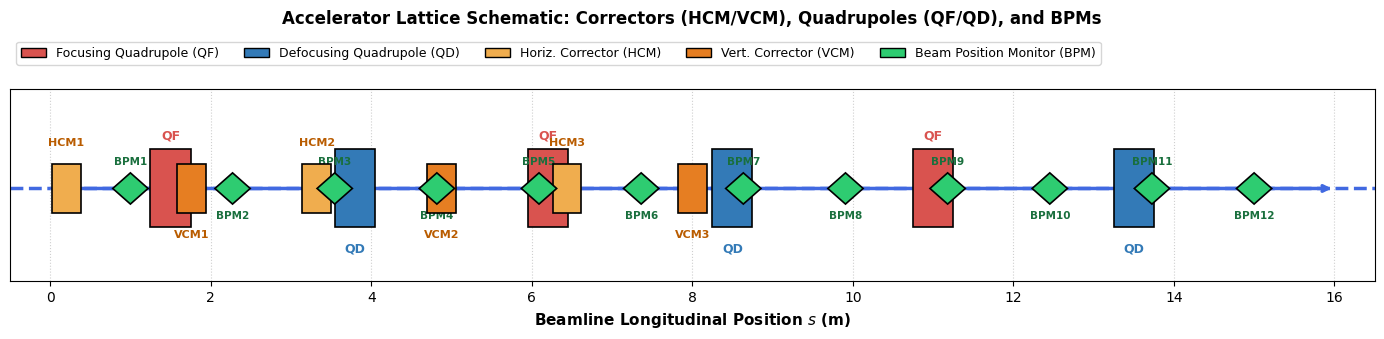
\includegraphics[width=0.95\textwidth]{beamline.png}
\caption{Schematic diagram of the 15-meter accelerator transport section showing alternating focusing (QF, red) and defocusing (QD, blue) quadrupoles, 6 dipole steerers (HCM/VCM), and 12 Beam Position Monitors.}
\label{fig:beamline}
\end{figure}

\subsection{Mini-Hackathon Lattice Geometry \& Realistic Non-Linearities}
The mini-hackathon benchmark lattice (Figure~\ref{fig:beamline}) models a 15-meter transport line:
\begin{itemize}
    \item \textbf{Actuators:} 6 dipole steerers (3 Horizontal `HCM1--3', 3 Vertical `VCM1--3') bounded in $[-5.0\text{ A}, +5.0\text{ A}]$, with single-step adjustments clipped to $[-0.8\text{ A}, +0.8\text{ A}]$.
    \item \textbf{Diagnostics:} 12 Beam Position Monitors ($s = 1.0\text{ m}$ to $15.0\text{ m}$) reading beam displacement in millimeters.
    \item \textbf{Magnetic Core Saturation:} Ferromagnetic saturation at higher excitation currents induces non-linear cubic rolloff:
    \begin{equation}
        \mathbf{Y}_{\text{sat}} = - 0.015 \cdot (\mathbf{I}^3 \cdot \mathbf{R})
    \end{equation}
    \item \textbf{Initial Misalignment Distortion ($\mathbf{Y}_0$):} Quadrupole displacement errors drawn per episode:
    \begin{equation}
        Y_{0, k} = A_1 \sin\left(\frac{2\pi s_k}{\lambda_1} + \phi_1\right) + A_2 \cos\left(\frac{2\pi s_k}{\lambda_2} + \phi_2\right)
    \end{equation}
    producing initial orbit errors between $0.4\text{ mm}$ and $1.1\text{ mm}$ RMS.
    \item \textbf{Gaussian Measurement Noise:} Sensor electronics introduce random noise $\boldsymbol{\epsilon} \sim \mathcal{N}(0, \sigma^2)$, with $\sigma = 0.010\text{ mm}$ ($10\ \mu\text{m}$).
\end{itemize}

The complete physical forward response equation is:
\begin{equation}
    \mathbf{Y} = \mathbf{I} \cdot \mathbf{R} - 0.015 \cdot (\mathbf{I}^3 \cdot \mathbf{R}) + \mathbf{Y}_0 + \boldsymbol{\epsilon}
\end{equation}

---

\section{Part 2: Machine Learning Fundamentals \& Neural Surrogate Modeling (25 min)}

\subsection{Machine Learning Taxonomy in Accelerators}
Machine Learning (ML) algorithms automatically extract functional mappings from numerical tracking simulations or machine archives without requiring explicit analytical re-derivation. In accelerator operations, ML encompasses three main paradigms:
\begin{itemize}
    \item \textbf{Supervised Learning:} Learning a continuous regression mapping $\mathbf{Y} = f(\mathbf{X})$ from actuator magnet currents $\mathbf{X}$ to beam diagnostic offsets $\mathbf{Y}$. This forms the foundation of \textbf{Surrogate Modeling / Digital Twins}.
    \item \textbf{Unsupervised Learning:} Uncovering latent structures in unlabelled data (e.g., PCA for betatron mode decomposition, autoencoders for anomaly detection).
    \item \textbf{Reinforcement Learning (RL):} Training an agent policy $\pi(a|s)$ through environmental interaction to maximize cumulative reward for \textbf{Autonomous Closed-Loop Control}.
\end{itemize}

\subsection{The Artificial Neuron: Mathematical Formulation}
The fundamental atom of a neural network is the \textbf{artificial neuron} (perceptron):
\begin{enumerate}
    \item \textbf{Linear Combination (Pre-Activation):}
    \begin{equation}
        z = \sum_{i=1}^n w_i x_i + b = \mathbf{w}^T \mathbf{x} + b
    \end{equation}
    where $\mathbf{w} \in \mathbb{R}^n$ denotes the trainable synaptic weights, $\mathbf{x} \in \mathbb{R}^n$ is the input feature vector, and $b \in \mathbb{R}$ is the scalar bias shifting the firing threshold.
    
    \item \textbf{Non-Linear Mapping (Post-Activation):}
    \begin{equation}
        a = \sigma(z) = \sigma(\mathbf{w}^T \mathbf{x} + b)
    \end{equation}
    where $\sigma(\cdot)$ is the activation function.
\end{enumerate}

\subsection{Why Non-Linear Activation Functions are Essential}
\begin{infobox}[The Collapse of Deep Linear Networks]
If all activation functions were linear identities ($\sigma(z) = z$), stacking $L$ sequential layers would yield:
\begin{equation}
    \hat{\mathbf{Y}} = \mathbf{W}_3 (\mathbf{W}_2 (\mathbf{W}_1 \mathbf{x} + \mathbf{b}_1) + \mathbf{b}_2) + \mathbf{b}_3 = (\mathbf{W}_3 \mathbf{W}_2 \mathbf{W}_1) \mathbf{x} + \mathbf{b}_{\text{net}} = \mathbf{W}_{\text{eff}} \mathbf{x} + \mathbf{b}_{\text{net}}
\end{equation}
A multi-layer linear network collapses mathematically into a \textbf{single linear matrix} $\mathbf{W}_{\text{eff}}$, offering no more expressive capacity than the classical linear Orbit Response Matrix $\mathbf{R}$.
\end{infobox}

Non-linear activation functions enable neural networks to act as Universal Function Approximators:
\begin{itemize}
    \item \textbf{Sigmoid:} $\sigma(z) = \frac{1}{1 + e^{-z}} \in (0, 1)$. Suffers from vanishing gradients when $|z| \gg 0$, halting weight updates during backpropagation.
    \item \textbf{Hyperbolic Tangent ($\tanh$):} $\tanh(z) = \frac{e^z - e^{-z}}{e^z + e^{-z}} \in (-1, 1)$. Zero-centered, but still prone to gradient saturation.
    \item \textbf{Rectified Linear Unit (ReLU):}
    \begin{equation}
        \text{ReLU}(z) = \max(0, z) = \begin{cases} z & \text{if } z > 0 \\ 0 & \text{if } z \le 0 \end{cases}
    \end{equation}
    \textbf{Why ReLU is standard in accelerator surrogates:}
    \begin{itemize}
        \item Constant unit derivative $\frac{d}{dz}\text{ReLU}(z) = 1.0$ for $z > 0$, completely preventing gradient vanishing.
        \item Extremely fast forward and backward passes without exponential function evaluation.
        \item Induces sparse representations by zeroing negative activations.
    \end{itemize}
\end{itemize}

\subsection{Multi-Layer Perceptron (MLP) Topology: Layers \& Information Flow}
A Multi-Layer Perceptron (MLP) organizes interconnected neurons into sequential layers:
\begin{itemize}
    \item \textbf{Input Layer ($\mathbb{R}^6$):} Ingests physical magnet actuator setpoints (the 6 corrector currents $I_1, \dots, I_6$).
    \item \textbf{Hidden Layers ($\mathbb{R}^{128} \rightarrow \mathbb{R}^{64} \rightarrow \mathbb{R}^{32}$):} Progressive hierarchical feature representations. Each layer computes:
    \begin{equation}
        \mathbf{h}^{(l)} = \text{ReLU}\left( \mathbf{W}^{(l)} \mathbf{h}^{(l-1)} + \mathbf{b}^{(l)} \right)
    \end{equation}
    \item \textbf{Output Layer ($\mathbb{R}^{12}$):} Linear projection predicting the 12 Beam Position Monitor readings ($\hat{Y}_1, \dots, \hat{Y}_{12}$).
\end{itemize}

\subsection{Loss Functions, Loss Rates \& Metrics: MSE vs.\ RMSE}
Network parameters are trained by minimizing an objective loss function:
\begin{enumerate}
    \item \textbf{Mean Squared Error (MSE) Loss:}
    \begin{equation}
        \mathcal{L}_{\text{MSE}}(\boldsymbol{\theta}) = \frac{1}{N \cdot M} \sum_{i=1}^N \sum_{j=1}^M \left( Y_{i,j} - \hat{Y}_{i,j}(\boldsymbol{\theta}) \right)^2
    \end{equation}
    Smoothly differentiable, penalizing large orbit outliers quadratically.
    
    \item \textbf{Root Mean Squared Error (RMSE) Evaluation Metric:}
    \begin{equation}
        \text{RMSE} = \sqrt{\mathcal{L}_{\text{MSE}}} = \sqrt{\frac{1}{N \cdot M} \sum_{i=1}^N \sum_{j=1}^M \left( Y_{i,j} - \hat{Y}_{i,j} \right)^2}
    \end{equation}
    \textbf{Why RMSE is the preferred metric in beam physics:} It preserves the original physical measurement units (\textbf{millimeters}) and directly reflects accelerator beam orbit distortion standards.
\end{enumerate}

\subsection{Optimization Algorithms: Gradient Descent \& The Adam Optimizer}
During backpropagation, loss gradients $\nabla_{\boldsymbol{\theta}} \mathcal{L}$ are propagated backward to update weights:
\begin{enumerate}
    \item \textbf{Stochastic Gradient Descent (SGD):} $\boldsymbol{\theta}_{t+1} = \boldsymbol{\theta}_t - \eta \nabla_{\boldsymbol{\theta}} \mathcal{L}$, where $\eta$ is the \textbf{learning rate}. High learning rates risk divergence; low learning rates cause stagnation.
    \item \textbf{The Adam Optimizer (Adaptive Moment Estimation):} Combines Momentum (first moment $\mathbf{m}_t$) and RMSprop (second moment $\mathbf{v}_t$):
    \begin{equation}
        \mathbf{m}_t = \beta_1 \mathbf{m}_{t-1} + (1-\beta_1) \mathbf{g}_t, \quad \mathbf{v}_t = \beta_2 \mathbf{v}_{t-1} + (1-\beta_2) \mathbf{g}_t^2
    \end{equation}
    \begin{equation}
        \hat{\mathbf{m}}_t = \frac{\mathbf{m}_t}{1-\beta_1^t}, \quad \hat{\mathbf{v}}_t = \frac{\mathbf{v}_t}{1-\beta_2^t} \implies \boldsymbol{\theta}_{t+1} = \boldsymbol{\theta}_t - \frac{\eta}{\sqrt{\hat{\mathbf{v}}_t} + \epsilon} \hat{\mathbf{m}}_t
    \end{equation}
    Adam automatically scales individual parameter updates, ensuring stable convergence across coupled magnet channels.
\end{enumerate}

\subsection{Dataset Partitioning \& The Bias-Variance Tradeoff}
To prevent memorization of diagnostic noise, data is partitioned into:
\begin{itemize}
    \item \textbf{Training Set (80\%, 1,200 shots):} Used directly for loss gradient computation and parameter updates.
    \item \textbf{Validation Set (Optional):} Monitored across epochs for early stopping before overfitting occurs.
    \item \textbf{Test / Holdout Set (20\%, 300 shots):} Strictly isolated during training to provide an unbiased benchmark on unseen accelerator states.
\end{itemize}
\begin{itemize}
    \item \textbf{Underfitting (High Bias):} Linear models cannot capture the cubic magnetic core saturation.
    \item \textbf{Overfitting (High Variance):} Over-parameterized models memorizing Gaussian sensor noise ($\sigma = 10\ \mu\text{m}$). Prevented using $L_2$ weight regularization (`alpha=1e-4`).
\end{itemize}

\subsection{Challenge Implementation \& Empirical Benchmark}
In Step 3 of the challenge notebook, $1,500$ experimental samples are synthesized uniformly across current boundaries $[-3.0\text{ A}, +3.0\text{ A}]$:
\begin{lstlisting}[language=Python]
n_train_samples = 1500
X_offline = np.random.uniform(-3.0, 3.0, size=(n_train_samples, env.n_correctors))
Y_linear = X_offline @ env.R
Y_sat = - 0.015 * (X_offline**3) @ env.R
bpm_noise = np.random.normal(0, 0.010, size=(n_train_samples, env.n_bpms))
Y_offline = Y_linear + Y_sat + bpm_noise

X_train, X_test, Y_train, Y_test = train_test_split(
    X_offline, Y_offline, test_size=0.20, random_state=42
)

# Train Linear Ridge vs Deep MLP Regressor
linear_model = Ridge(alpha=1.0).fit(X_train, Y_train)
surrogate_model = MLPRegressor(
    hidden_layer_sizes=(128, 64, 32), activation='relu',
    solver='adam', alpha=1e-4, max_iter=400, random_state=42
).fit(X_train, Y_train)
\end{lstlisting}

\begin{table}[h!]
\centering
\resizebox{\textwidth}{!}{%
\begin{tabular}{@{}lcccp{6.5cm}@{}}
\toprule
\textbf{Model Architecture} & \textbf{Parameters} & \textbf{Holdout RMSE} & \textbf{Inference Latency} & \textbf{Physical Regimes Captured} \\
\midrule
Linear Ridge Baseline ($\lambda=1.0$) & 72 & $0.0558\text{ mm}$ & $< 0.01\text{ ms}$ & Linear optics only; misses saturation. \\
MLP Neural Surrogate & 11,596 & $\mathbf{0.0118\text{ mm}}$ & $\approx 0.15\text{ ms}$ & Linear ORM and cubic saturation down to noise floor. \\
\bottomrule
\end{tabular}%
}
\caption{Holdout validation performance on 20\% test partition (300 unseen shots).}
\label{tab:surrogate_perf}
\end{table}

\begin{infobox}[Physical Insight: The Bayesian Sensor Noise Floor]
The holdout error of the MLP ($0.0118\text{ mm}$) closely approaches the theoretical noise floor set by Gaussian BPM sensor jitter ($\sigma = 0.0100\text{ mm}$). This indicates that the neural surrogate has learned the non-linear physics without overfitting sensor noise.
\end{infobox}

---

\section{Part 3: Closed-Loop Control Paradigms (25 min)}

\subsection{Baseline 0: Classical SVD Pseudo-Inverse Controller}
In standard accelerator control rooms, Singular Value Decomposition (SVD) of the transpose response matrix $\mathbf{R}^T = \mathbf{U} \boldsymbol{\Sigma} \mathbf{V}^T$ provides the Moore-Penrose pseudo-inverse:
\begin{equation}
    (\mathbf{R}^T)^\dagger = \mathbf{V} \boldsymbol{\Sigma}^{-1} \mathbf{U}^T
\end{equation}
The closed-loop correction action per step is:
\begin{equation}
    \Delta \mathbf{I} = \text{clip}\left( - \alpha \cdot (\mathbf{R}^T)^\dagger \cdot \mathbf{Y}_{\text{obs}}, \ -0.8, \ +0.8 \right)
\end{equation}
where $\alpha \approx 0.45$ is the feedback gain.
While computationally instantaneous, SVD assumes linearity; when correctors saturate, high gains trigger overshooting and limit-cycle oscillations.

\subsection{Baseline 1: Model-Based Optimization via Digital Twin Inversion}
Rather than inverting an analytical matrix, Baseline 1 optimizes corrective kicks directly through the forward neural surrogate $f_{\boldsymbol{\theta}}(\Delta \mathbf{I})$ using SciPy's \texttt{L-BFGS-B} algorithm:
\begin{equation}
    \min_{\Delta \mathbf{I}} \mathcal{L}(\Delta \mathbf{I}) = \left\| \mathbf{Y}_{\text{obs}} + f_{\boldsymbol{\theta}}(\Delta \mathbf{I}) \right\|_2^2 + \lambda \|\Delta \mathbf{I}\|_2^2 \quad \text{s.t.} \quad \Delta \mathbf{I} \in [-5.0\text{ A}, +5.0\text{ A}]^6
\end{equation}

\begin{lstlisting}[language=Python]
class SupervisedMLPController:
    def __init__(self, surrogate):
        self.surrogate = surrogate

    def act(self, obs, info=None):
        def objective(delta_I):
            pred = self.surrogate.predict(delta_I.reshape(1, -1))[0]
            residual = obs + pred
            return np.sum(residual**2) + 0.0001 * np.sum(delta_I**2)
            
        res = opt.minimize(objective, np.zeros(6), bounds=[(-5.0, 5.0)]*6, method='L-BFGS-B')
        return np.clip(res.x, -0.8, 0.8)
\end{lstlisting}
Because the surrogate anticipates non-linear saturation falloff, Baseline 1 reaches convergence in only \textbf{2 to 3 iterations}.

\subsection{Track 2: Closed-Loop RL Policy with Physics Prior and Adaptive Damping}
Model-based iterative optimization requires $15$--$30\text{ ms}$ per step. A closed-loop policy network executes in $< 0.5\text{ ms}$.
High-performing accelerator policy agents integrate an analytical **physics prior** with a learned parameter residual and dynamic step damping:
\begin{equation}
    \Delta \mathbf{I}(t) = \gamma(t) \cdot \left[ \underbrace{- \alpha (\mathbf{R}^T)^\dagger \mathbf{Y}}_{\text{Analytical Physics Prior}} + \underbrace{\mathbf{W}_{\text{learned}}\mathbf{Y} + \mathbf{b}}_{\text{Learned Residual Offset}} \right]
\end{equation}
\begin{equation}
    \gamma(t) = \frac{1.0}{1.0 + 0.03 \cdot t}
\end{equation}
The dynamic damping factor $\gamma(t)$ decays control authority as the beam approaches the $0.030\text{ mm}$ boundary, preventing sensor noise amplification from destabilizing the closed orbit.

---

\section{Part 4: Mini-Hackathon Problem Formulation \& Gymnasium Contract (15 min)}

\subsection{Gymnasium Environment Specification (\texttt{AcceleratorOrbitGymEnv})}
\begin{itemize}
    \item \textbf{Observation Space:} $\text{Box}(-10.0, +10.0, \text{shape}=(12,), \text{dtype}=\text{float32})$ (BPM readings in mm).
    \item \textbf{Action Space:} $\text{Box}(-0.8, +0.8, \text{shape}=(6,), \text{dtype}=\text{float32})$ (Incremental kicks $\Delta \mathbf{I}$ in Amperes).
    \item \textbf{State Update:} $\mathbf{I}_{t+1} = \text{clip}(\mathbf{I}_t + \Delta \mathbf{I}_t, -5.0, 5.0)$.
    \item \textbf{Reward Function:}
    \begin{equation}
        r_t = - \text{RMS}_{t+1} - 0.01 \cdot \|\Delta \mathbf{I}_t\|_2 + (50.0 \text{ if } \text{RMS}_{t+1} < 0.030\text{ mm} \text{ else } 0.0)
    \end{equation}
    \item \textbf{Success Criteria:} Terminated when $\text{RMS} < 0.030\text{ mm}$; truncated if step count reaches $20$.
\end{itemize}

\subsection{Standardized 30-Seed Evaluation \& Official Scoring Formula}
Controllers are evaluated across 30 standardized seeds (\texttt{range(1, 31)}). The official benchmark score is defined as:
\begin{equation}
    \text{Score} = (\text{Success Rate} \times 10.0) - (2.0 \times \overline{\text{Steps}}) + \left(\frac{0.03}{\max(\overline{\text{RMS}}, 0.005)} \times 20.0\right) - (2.0 \times \overline{\|\mathbf{I}\|})
\end{equation}

\begin{table}[h!]
\centering
\resizebox{\textwidth}{!}{%
\begin{tabular}{@{}clccccc@{}}
\toprule
\textbf{Rank} & \textbf{Controller Paradigm} & \textbf{Success Rate} & \textbf{Mean Steps} & \textbf{Final RMS} & \textbf{Current Norm} & \textbf{Official Score} \\
\midrule
\textbf{\#1} & Baseline 1: Supervised MLP Inversion & 100.0\% & \textbf{2.3 steps} & $0.0257\text{ mm}$ & $1.21\text{ A}$ & \textbf{1,016.8 pts} \\
\textbf{\#2} & Baseline 0: Classical Linear SVD & 100.0\% & 5.6 steps & \textbf{0.0230 mm} & \textbf{1.16 A} & \textbf{1,013.1 pts} \\
\textbf{\#3} & Track 2: Closed-Loop RL Policy & 100.0\% & 6.1 steps & $0.0239\text{ mm}$ & $1.18\text{ A} $& \textbf{1,011.1 pts} \\
\bottomrule
\end{tabular}%
}
\caption{Official benchmark results across 30 evaluation seeds.}
\label{tab:leaderboard}
\end{table}

---

\section{Part 5: Summary, Q\&A \& Transition to Lecture 2 (5 min)}

\begin{infobox}[Summary Takeaways]
\begin{enumerate}
    \item \textbf{Physics-Informed Prior:} Initializing AI policies with the analytical pseudo-inverse ORM guarantees early stability and avoids millions of exploratory random steps.
    \item \textbf{Non-Linear Representation:} Deep neural surrogates bridge the gap between idealized linear beam optics and real-world magnetic saturation.
    \item \textbf{Dynamic Step Damping:} Attenuating feedback near diagnostic noise floors prevents terminal limit cycles and ensures robust convergence.
\end{enumerate}
\end{infobox}

\textbf{Next Session:} Dr.~Thorsten Hellert will present \textit{Agentic AI for Accelerator Research: Osprey Applications} (10:40 -- 12:00), exploring LLM agents, automated tool calling, and autonomous accelerator orchestration.

\vspace{1.5em}
\noindent\textbf{References:}
\begin{small}
\begin{enumerate}
    \item Minty, M. G., \& Zimmermann, F. (2003). \textit{Measurement and Control of Charged Particle Beams}. Springer.
    \item Wiedemann, H. (2015). \textit{Particle Accelerator Physics} (4th ed.). Springer.
    \item Hellert, T., et al. (2024). \textit{Autonomous Accelerator Tuning using Large Language Model Agents and Osprey}. Phys. Rev. Accel. Beams.
    \item Edelen, A., et al. (2020). \textit{Machine learning for orders-of-magnitude speedup in multiobjective optimization of particle accelerator beamlines}. Phys. Rev. Accel. Beams, 23(4), 044601.
\end{enumerate}
\end{small}

\end{document}
